\documentclass{article}
\usepackage[T1]{fontenc}
\usepackage{lmodern}
\usepackage{graphicx}
\usepackage{amsmath,amssymb}
\usepackage[a4paper,margin=2cm]{geometry}
\usepackage[absolute,overlay]{textpos}
\setlength{\TPHorizModule}{1mm}
\setlength{\TPVertModule}{1mm}
\usepackage[indonesian]{babel}
\usepackage{hyperref}
\setlength{\emergencystretch}{2em}
% unit: Halaman 33

\begin{document}

% === Halaman 33 (python/native) ===

33

Kelemahan Mode CBC

1. Kesalahan  satu bit pada sebuah blok 

plainteks akan menghasilkan kesalahan  

pada blok cipherteks yang berkoresponden 

dan kesalahan tersebut merambat ke 

semua blok cipherteks berikutnya.

2.  Tetapi, hal ini berkebalikan pada proses 

dekripsi. Kesalahan satu bit pada blok 

cipherteks hanya mempengaruhi blok 

plainteks yang berkoresponden dan satu 

bit pada blok plainteks berikutnya (pada 

posisi bit yang berkoresponden pula).

% deskripsi: gambar native xref 126
\noindent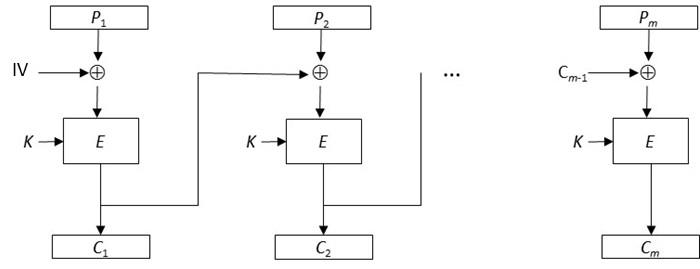
\includegraphics[width=0.85\textwidth]{../../images/python/page_033_img_01.jpeg}

% deskripsi: gambar native xref 127
\noindent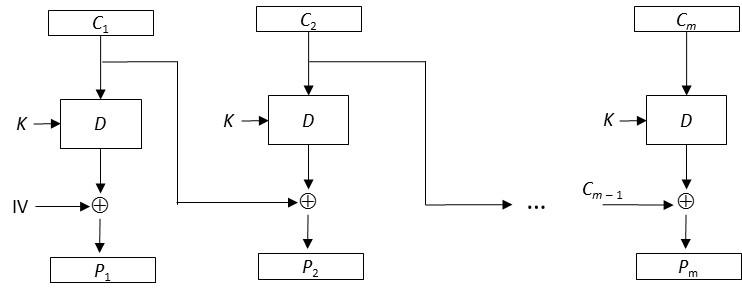
\includegraphics[width=0.85\textwidth]{../../images/python/page_033_img_02.jpeg}

\end{document}
